\section{Phương pháp lưới}

\subsection{Giới thiệu về lưới}
%%%%%%%%%%%%%%%%%%%%%%%%%%%%%%%%%%%%%%%%%%%%%%%%%%%%%%%
% Nguồn Survey: Lattice Reduction Attacks on RSA; David Wong; supervised by Guilhem Castagnos; University of Bordeaux, March 2015
\begin{frame}{Giới thiệu về lưới}

\begin{itemize}
\item Ta có thể hiểu lưới tương tự như không gian vector
\item Ví dụ không gian vector đơn giản gồm 2 vector

\begin{itemize}
\item Bạn có thể cộng vector, nhân vô hướng với 1 số
% \item Kết quả trải rộng trong một không gian vector.
\end{itemize}
\end{itemize}

% \begin{figure}[!h]
\resizebox{0.9\textwidth}{!}{%

\begin{tikzpicture}[scale=.5]
\draw [lightgray] [<->] (0, 5) -- (10, 5);
\draw [lightgray] [<->] (5, 10) -- (5, 0);
\draw [thick, purple] [->] (5, 5) -- (6, 8);
\draw [thick, purple] [->] (5, 5) -- (6, 6);

\draw [thick, black] [->] (11, 5) -- (12, 5);

\draw [lightgray] [<->] (13, 5) -- (23, 5);
\draw [lightgray] [<->] (18, 10) -- (18, 0);
\path [fill=purple] (15.5, 0) to (20.5, 10) to (23, 10) to (13, 0);
\end{tikzpicture}
}
% \end{figure}

\end{frame}
%%%%%%%%%%%%%%%%%%%%%%%%%%%%%%%%%%%%%%%%%%%%%%%%%%%%%%%
% Nguồn Survey: Lattice Reduction Attacks on RSA; David Wong; supervised by Guilhem Castagnos; University of Bordeaux, March 2015
\begin{frame}{Giới thiệu về lưới}

\begin{itemize}
\item Tuy nhiên, các số vô hướng của lưới là các số nguyên
\item Bây giờ ta có không gian được tạo thành từ các điểm
\item Đặc điểm của không gian này là có tính rời rạc
\end{itemize}

\begin{figure}[!h]
\centering
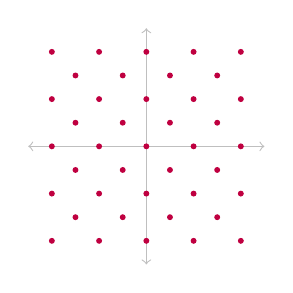
\begin{tikzpicture}[scale=.3]
\draw [lightgray] [<->] (0, 5) -- (10, 5);
\draw [lightgray] [<->] (5, 10) -- (5, 0);

\draw [fill, purple] (9, 1) circle [radius=0.1];

\draw [fill, purple] (7, 1) circle [radius=0.1];
\draw [fill, purple] (8, 2) circle [radius=0.1];
\draw [fill, purple] (9, 3) circle [radius=0.1];

\draw [fill, purple] (5, 1) circle [radius=0.1];
\draw [fill, purple] (6, 2) circle [radius=0.1];
\draw [fill, purple] (7, 3) circle [radius=0.1];
\draw [fill, purple] (8, 4) circle [radius=0.1];
\draw [fill, purple] (9, 5) circle [radius=0.1];

\draw [fill, purple] (3, 1) circle [radius=0.1];
\draw [fill, purple] (4, 2) circle [radius=0.1];
\draw [fill, purple] (5, 3) circle [radius=0.1];
\draw [fill, purple] (6, 4) circle [radius=0.1];
\draw [fill, purple] (7, 5) circle [radius=0.1];
\draw [fill, purple] (8, 6) circle [radius=0.1];
\draw [fill, purple] (9, 7) circle [radius=0.1];

\draw [fill, purple] (1, 1) circle [radius=0.1];
\draw [fill, purple] (2, 2) circle [radius=0.1];
\draw [fill, purple] (3, 3) circle [radius=0.1];
\draw [fill, purple] (4, 4) circle [radius=0.1];
\draw [fill, purple] (5, 5) circle [radius=0.1];
\draw [fill, purple] (6, 6) circle [radius=0.1];
\draw [fill, purple] (7, 7) circle [radius=0.1];
\draw [fill, purple] (8, 8) circle [radius=0.1];
\draw [fill, purple] (9, 9) circle [radius=0.1];

\draw [fill, purple] (1, 3) circle [radius=0.1];
\draw [fill, purple] (2, 4) circle [radius=0.1];
\draw [fill, purple] (3, 5) circle [radius=0.1];
\draw [fill, purple] (4, 6) circle [radius=0.1];
\draw [fill, purple] (5, 7) circle [radius=0.1];
\draw [fill, purple] (6, 8) circle [radius=0.1];
\draw [fill, purple] (7, 9) circle [radius=0.1];

\draw [fill, purple] (1, 5) circle [radius=0.1];
\draw [fill, purple] (2, 6) circle [radius=0.1];
\draw [fill, purple] (3, 7) circle [radius=0.1];
\draw [fill, purple] (4, 8) circle [radius=0.1];
\draw [fill, purple] (5, 9) circle [radius=0.1];

\draw [fill, purple] (1, 7) circle [radius=0.1];
\draw [fill, purple] (2, 8) circle [radius=0.1];
\draw [fill, purple] (3, 9) circle [radius=0.1];

\draw [fill, purple] (1, 9) circle [radius=0.1];
\end{tikzpicture}
\end{figure}

\begin{block}{Nhận xét}
Lưới rất hữu ích trong mật mã vì chúng mang lại cho chúng ta rất nhiều công cụ để xử lý các số nguyên
\end{block}

\end{frame}
%%%%%%%%%%%%%%%%%%%%%%%%%%%%%%%%%%%%%%%%%%%%%%%%%%%%%%%
% \subsection{Định nghĩa}
% \begin{frame}{Định nghĩa}
% \begin{block}{Tập hợp các vector độc lập tuyến tính}
% Tập hợp các vector \(\{x_1, x_2, \ldots, x_n\}\) trong \(\mathbb{R}^n\) độc lập tuyến tính nếu:

% \begin{equation}
% c_1 x_1 + c_2 x_2 + \ldots + c_n x_n = 0 \quad \text{với} \quad c_i \in \mathbb{R}
% \end{equation}

% Dấu "=" xảy ra khi và chỉ khi \(c_1 = c_2 = \ldots = c_n = 0 \).

% \end{block}
% \end{frame}
%%%%%%%%%%%%%%%%%%%%%%%%%%%%%%%%%%%%%%%%%%%%%%%%%%%%%%%
\subsection{Định nghĩa lưới}

\begin{frame}{Định nghĩa lưới}

\begin{block}{Định nghĩa lưới}

Cho \(n \geq 1 \), \(\{x_1, x_2, \ldots, x_n\}\) là một cơ sở của \(\mathbb{R}^n\).
Lưới \(n \) chiều với cơ sở \(\{x_1, x_2, \ldots, x_n\}\)
là tập hợp tất cả các tổ hợp tuyến tính của các vector cơ sở đó với hệ số nguyên:

$$
L = \{a_1 x_1 + a_2 x_2 + \ldots + a_n x_n \mid a_i \in \mathbb{Z} \}
$$

Trong đó các vector \(\{x_1, x_2, \ldots, x_n\}\) được gọi là cơ sở của lưới.

\end{block}

\end{frame}
%%%%%%%%%%%%%%%%%%%%%%%%%%%%%%%%%%%%%%%%%%%%%%%%%%%%%%%
\begin{frame}{Ví dụ về lưới 2 chiều}

\begin{figure}[!h]
\centering
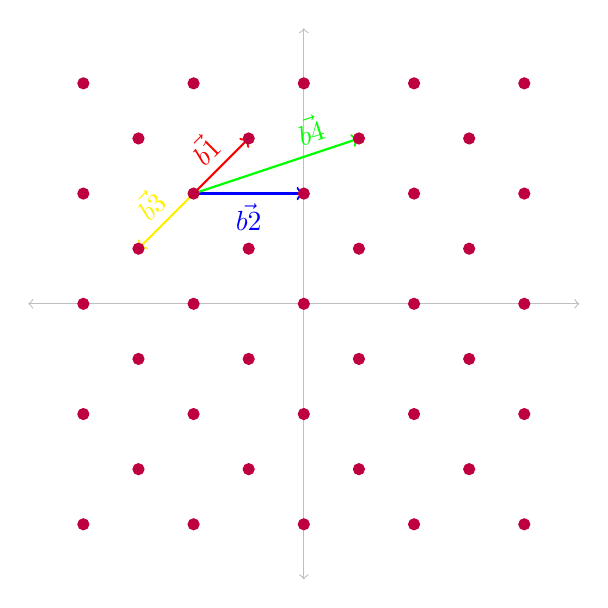
\begin{tikzpicture}[scale=.7]
\draw [lightgray] [<->] (0, 5) -- (10, 5);
\draw [lightgray] [<->] (5, 10) -- (5, 0);

\draw[->, thick, red] (3, 7) -- (4, 8) node[midway, above, sloped] {$\vec{b1}$};
\draw[->, thick, blue] (3, 7) -- (5, 7) node[midway, below, sloped] {$\vec{b2}$};
\draw[->, thick, yellow] (3, 7) -- (2, 6) node[midway, above, sloped] {$\vec{b3}$};
\draw[->, thick, green] (3, 7) -- (6, 8) node[pos=0.75, above, sloped] {$\vec{b4}$};

\draw [fill, purple] (9, 1) circle [radius=0.1];

\draw [fill, purple] (7, 1) circle [radius=0.1];
\draw [fill, purple] (8, 2) circle [radius=0.1];
\draw [fill, purple] (9, 3) circle [radius=0.1];

\draw [fill, purple] (5, 1) circle [radius=0.1];
\draw [fill, purple] (6, 2) circle [radius=0.1];
\draw [fill, purple] (7, 3) circle [radius=0.1];
\draw [fill, purple] (8, 4) circle [radius=0.1];
\draw [fill, purple] (9, 5) circle [radius=0.1];

\draw [fill, purple] (3, 1) circle [radius=0.1];
\draw [fill, purple] (4, 2) circle [radius=0.1];
\draw [fill, purple] (5, 3) circle [radius=0.1];
\draw [fill, purple] (6, 4) circle [radius=0.1];
\draw [fill, purple] (7, 5) circle [radius=0.1];
\draw [fill, purple] (8, 6) circle [radius=0.1];
\draw [fill, purple] (9, 7) circle [radius=0.1];

\draw [fill, purple] (1, 1) circle [radius=0.1];
\draw [fill, purple] (2, 2) circle [radius=0.1];
\draw [fill, purple] (3, 3) circle [radius=0.1];
\draw [fill, purple] (4, 4) circle [radius=0.1];
\draw [fill, purple] (5, 5) circle [radius=0.1];
\draw [fill, purple] (6, 6) circle [radius=0.1];
\draw [fill, purple] (7, 7) circle [radius=0.1];
\draw [fill, purple] (8, 8) circle [radius=0.1];
\draw [fill, purple] (9, 9) circle [radius=0.1];

\draw [fill, purple] (1, 3) circle [radius=0.1];
\draw [fill, purple] (2, 4) circle [radius=0.1];
\draw [fill, purple] (3, 5) circle [radius=0.1];
\draw [fill, purple] (4, 6) circle [radius=0.1];
\draw [fill, purple] (5, 7) circle [radius=0.1];
\draw [fill, purple] (6, 8) circle [radius=0.1];
\draw [fill, purple] (7, 9) circle [radius=0.1];

\draw [fill, purple] (1, 5) circle [radius=0.1];
\draw [fill, purple] (2, 6) circle [radius=0.1];
\draw [fill, purple] (3, 7) circle [radius=0.1];
\draw [fill, purple] (4, 8) circle [radius=0.1];
\draw [fill, purple] (5, 9) circle [radius=0.1];

\draw [fill, purple] (1, 7) circle [radius=0.1];
\draw [fill, purple] (2, 8) circle [radius=0.1];
\draw [fill, purple] (3, 9) circle [radius=0.1];

\draw [fill, purple] (1, 9) circle [radius=0.1];
\end{tikzpicture}
\end{figure}

\end{frame}
%%%%%%%%%%%%%%%%%%%%%%%%%%%%%%%%%%%%%%%%%%%%%%%%%%%%%%%
\begin{frame}{Định thức}
\begin{block}{Định thức}

Với $\{x_1, x_2, \dots, x_n\} $ là cơ sở của lưới $L$ ta định nghĩa $$det L = |det(x_1, x_2, \dots, x_n)|$$
Về hình học, nó là thể tích của các hình bình hành kéo dài bởi các vector cơ sở $x_1, x_2, \dots, x_n$.

\end{block}
\end{frame}
%%%%%%%%%%%%%%%%%%%%%%%%%%%%%%%%%%%%%%%%%%%%%%%%%%%%%%%
\begin{frame}{Bổ đề}
\begin{block}{Bổ đề}
Cho $x_1, x_2, \ldots, x_n$ và $y_1, y_2, \ldots, y_n$ là hai cơ sở của lưới $L \subset \mathbb{R}^n$.
Lấy $X$, $Y$ lần lượt là các ma trận $n \times n$ nhận $x_i$ (tương ứng $y_i$) là các hàng thứ $i$.
Khi đó:

\begin{equation} \label{equation:bo_de}
Y = CX
\end{equation}

với $C$ là ma trận vuông $n \times n$ với các hệ số nguyên
và $\det(C) = \pm 1$.
\end{block}
\end{frame}
%%%%%%%%%%%%%%%%%%%%%%%%%%%%%%%%%%%%%%%%%%%%%%%%%%%%%%%
\begin{frame}{Bổ đề}

\textbf{Chứng minh:}

Với mọi $y_i$ thuộc lưới với cơ sở $x_1, x_2, \ldots, x_n$ và mọi $x_i$ thuộc lưới với cơ sở $y_1, y_2, \ldots, y_n$. Khi đó:
\[
x_i = \sum_{j=1}^n b_{ij} y_j, \quad y_i = \sum_{j=1}^n c_{ij} x_j.
\]

Ta có thể viết gọn lại dưới dạng ma trận:
$X = BY, \quad Y = CX.$

Vì vậy ta có $X = BCX$ và $Y = CBY$.

% Do $x_1, x_2, \ldots, x_n$ và $y_1, y_2, \ldots, y_n$
% là cơ sở trong không gian $\mathbb{R}^n$
% nên ma trận $X$, $Y$ là ma trận khả nghịch.

Suy ra $BC = CB = I$ và $\det(B) \det(C) = 1$.

Thêm nữa, $B$, $C$ là các ma trận hệ số nguyên. Do đó:
$$\det(B) = \det(C) = \pm 1$$

\end{frame}
%%%%%%%%%%%%%%%%%%%%%%%%%%%%%%%%%%%%%%%%%%%%%%%%%%%%%%%
\begin{frame}{Nhận xét}

\begin{block}{Nhận xét}
Định thức của một lưới không phụ thuộc vào cách chọn cơ sở.
\end{block}

\textbf{Chứng minh:}

Giả sử lưới $L \subset \mathbb{R}^n$ có 2 cơ sở $x_1, x_2, \ldots, x_n$ và $y_1, y_2, \ldots, y_n$.

Theo công thức (\ref{equation:bo_de}) trong bổ đề, ta có:

\[
|\det(Y)| = |\det(CX)| = |\det(C) \cdot \det(X)| = |\pm 1 \cdot \det(X)| = |\det(X)|
\]

\end{frame}
%%%%%%%%%%%%%%%%%%%%%%%%%%%%%%%%%%%%%%%%%%%%%%%%%%%%%%%
\subsection{Quy trình Gram-Schmidt}
\begin{frame}{Quy trình Gram-Schmidt}

\begin{itemize}
\item Quy trình Gram-Schmidt chuyển một cơ sở bất kỳ thành một cơ sở trực giao.
\item Đây là kỹ thuật quan trọng trong thuật toán LLL.
\end{itemize}

\begin{columns}

\begin{column}{0.5\textwidth}
\begin{figure}[h]

\resizebox{0.9\textwidth}{!}{%

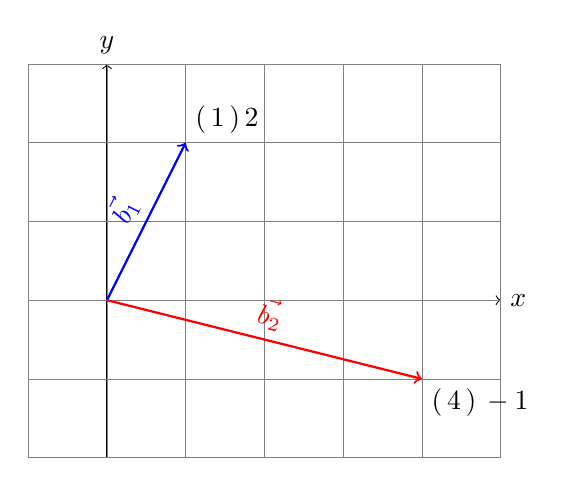
\begin{tikzpicture}
% Vẽ trục tọa độ
\draw[->] (-1, 0) -- (5, 0) node[right] {$x$};
\draw[->] (0, -2) -- (0, 3) node[above] {$y$};

% Vẽ lưới
\draw[very thin, gray] (-1, -2) grid (5, 3);

% Vẽ vector (1, 2)
\draw[->, thick, blue] (0, 0) -- (1, 2) node[midway, above, sloped] {$\vec{b_1}$};

% Vẽ vector (4, -1)
\draw[->, thick, red] (0, 0) -- (4, -1) node[midway, above, sloped] {$\vec{b_2}$};

% Gắn nhãn điểm cuối vector
\node at (1, 2) [above right] {$\begin{pmatrix} 1 \\ 2 \end{pmatrix}$};
\node at (4, -1) [below right] {$\begin{pmatrix} 4 \\ -1 \end{pmatrix}$};
\end{tikzpicture}

}

\end{figure}
\end{column}

\begin{column}{0.5\textwidth}
\begin{figure}[h]

\resizebox{0.9\textwidth}{!}{%

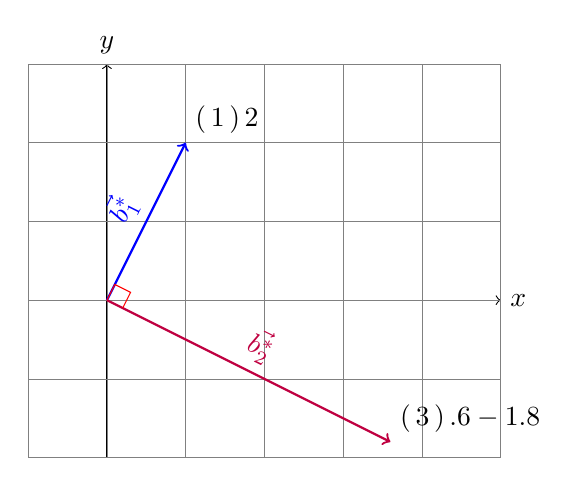
\begin{tikzpicture}
% Vẽ trục tọa độ
\draw[->] (-1, 0) -- (5, 0) node[right] {$x$};
\draw[->] (0, -2) -- (0, 3) node[above] {$y$};

% Vẽ lưới
\draw[very thin, gray] (-1, -2) grid (5, 3);

% Vẽ vector (1, 2)
\draw[->, thick, blue] (0, 0) -- (1, 2) node[midway, above, sloped] {$\vec{b_1^*}$};

% Vẽ vector (3.6, -1.8)
\draw[->, thick, purple] (0, 0) -- (3.6, -1.8) node[midway, above, sloped] {$\vec{b_2^*}$};

% Gắn nhãn điểm cuối vector
\node at (1, 2) [above right] {$\begin{pmatrix} 1 \\ 2 \end{pmatrix}$};
\node at (3.6, -1.8) [above right] {$\begin{pmatrix} 3.6 \\ -1.8 \end{pmatrix}$};

% Vẽ ký hiệu vuông góc màu đỏ tại gốc tọa độ
\draw[red] (0, 0) -- (0.1, 0.2) -- (0.3, 0.1) -- (0.2, -0.1);
\end{tikzpicture}

}

\end{figure}
\end{column}

\end{columns}

\end{frame}
%%%%%%%%%%%%%%%%%%%%%%%%%%%%%%%%%%%%%%%%%%%%%%%%%%%%%%%
\begin{frame}{Quy trình Gram-Schmidt}

\begin{block}{Định nghĩa}

Cho $x_1, x_2, \ldots, x_n$ là một cơ sở trong $\mathbb{R}^n$.
Trực giao hóa Gram-Schmidt của $x_1, x_2, \ldots, x_n$
là một cơ sở $x_1^*, x_2^*, \ldots, x_n^*$ được định nghĩa như sau:

\begin{itemize}
\item $x_1 = x_1^*$,
\item $x_i^* = x_i - \sum_{j=1}^{i-1} \mu_{ij} x_j^*$, \quad $2 \leq i \leq n$, \quad $\mu_{ij} = \frac{\langle x_i, x_j^* \rangle}{\langle x_j^*, x_j^* \rangle}$.
\end{itemize}

\end{block}

\end{frame}
%%%%%%%%%%%%%%%%%%%%%%%%%%%%%%%%%%%%%%%%%%%%%%%%%%%%%%%
\begin{frame}{Nhận xét quy trình Gram-Schmidt}

\begin{itemize}
\item Các vector không được chuẩn hóa độ dài

\item Nếu $x_1, x_2, \dots, x_n$ là một cơ sở của lưới $L$ thì sau khi trực giao hóa ta thu được các vector $x_1^*, x_2^*, \dots, x_n^*$ có thể không nằm trong lưới $L$.
\item Để đảm bảo tạo ra một cơ sở "đủ trực giao" trong lưới, chúng ta cần $\mu_{ij}$ là một số nguyên.

% Nếu ta đặt $\mu_{ii} = 1 $, $\mu_{ij} = 0$ với $ 1\leq i < j \leq n$ .
\item Ta có thể viết lại $x_i^* = x_i - \sum_{j=1}^{i-1} \mu_{ij} x_j^*$ dưới dạng ma trận:
$$\underbrace{\left(\begin{array}{c}
x_1 \\
x_2 \\
\vdots \\
x_n
\end{array}\right)}_{X} = \underbrace{\left(\begin{array}{cccc}
1 & 0 & \cdots & 0 \\
\mu_{21} & 1 & \cdots & 0 \\
\vdots & \vdots & \ddots & \vdots \\
\mu_{n1} & \cdots & \cdots & 1
\end{array}\right)}_{M} \times \underbrace{\left(\begin{array}{c}
x_1^* \\
x_2^* \\
\vdots \\
x_n^*
\end{array}\right)}_{X^*} $$

\end{itemize}

\end{frame}
%%%%%%%%%%%%%%%%%%%%%%%%%%%%%%%%%%%%%%%%%%%%%%%%%%%%%%%
\begin{frame}{Định lý}

\begin{block}{Định lý}

Cho $x_1, x_2, \ldots, x_n$ là một cơ sở của $\mathbb{R}^n$
và $x_1^*, x_2^*, \ldots, x_n^*$ là trực giao hóa Gram-Schmidt của nó. Khi đó:

\begin{equation} \label{equation:dinh_li_Gram-Schmidt1}
\langle x_i^*, x_j^* \rangle = 0 \quad \text{với} \quad 1 \leq i < j \leq n
\end{equation}

\begin{equation} \label{equation:dinh_li_Gram-Schmidt2}
\|x_k^*\| \leq \|x_k\|
\end{equation}

\begin{equation} \label{equation:dinh_li_Gram-Schmidt3}
\det(X^*) = \det(X)
\end{equation}

\end{block}

\end{frame}
%%%%%%%%%%%%%%%%%%%%%%%%%%%%%%%%%%%%%%%%%%%%%%%%%%%%%%%
\begin{frame}{Định lý}

\textbf{Chứng minh công thức (\ref{equation:dinh_li_Gram-Schmidt1}):}
$\langle x_i^*, x_j^* \rangle = 0$ với $1 \leq i < j \leq n$

Theo định nghĩa của quá trình trực giao hóa Gram-Schmidt,
các vector $x_1^*, x_2^*, \ldots, x_n^*$ được xây dựng sao cho
mỗi vector mới là trực giao với tất cả các vector trước đó.
Cụ thể, với $x_i^*$ và $x_j^*$:

\[
x_j^* = x_j - \sum_{k=1}^{j-1} \mu_{jk} x_k^*, \quad \text{với} \quad \mu_{jk} = \frac{\langle x_j, x_k^* \rangle}{\langle x_k^*, x_k^* \rangle}
\]

Do đó, $ x_i^* x_j^* = 0$ với $1 \leq i < j \leq n$.

\end{frame}
%%%%%%%%%%%%%%%%%%%%%%%%%%%%%%%%%%%%%%%%%%%%%%%%%%%%%%%
\begin{frame}{Định lý}

\textbf{Chứng minh công thức (\ref{equation:dinh_li_Gram-Schmidt2}):}
$\|x_k^*\| \leq \|x_k\|$

Do $x_i^*$ là hình chiếu của $x_i$ lên không gian trực giao với các vector trước đó, ta có:

\[
x_i^* = x_i - \sum_{j=1}^{i-1} \mu_{ij} x_j^*
\]

Theo định lý Py-ta-go, ta có:

\[
\|x_k\|^2 = \|x_k^*\|^2 + \sum_{j=1}^{k-1} (\mu_{kj})^2 \|x_j^*\|^2.
\]

Do đó, $\|x_i^*\| \leq \|x_i\|$.

\end{frame}
%%%%%%%%%%%%%%%%%%%%%%%%%%%%%%%%%%%%%%%%%%%%%%%%%%%%%%%
\begin{frame}{Định lý}

\textbf{Chứng minh công thức (\ref{equation:dinh_li_Gram-Schmidt3}):}
$\det(X^*) = \det(X)$

Theo quá trình Gram-Schmidt, ta có $X = MX^*$
với $M$ là ma trận tam giác dưới với các phần tử đường chéo bằng 1 và các phần tử dưới đường chéo chính là các hệ số $\mu_{ij}$.
Ma trận $M$ có định thức bằng 1, do đó:

\[
\det(X) = \det(MX^*) = \det(M) \det(X^*) = 1 \cdot \det(X^*) = \det(X^*)
\]

\end{frame}
%%%%%%%%%%%%%%%%%%%%%%%%%%%%%%%%%%%%%%%%%%%%%%%%%%%%%%%
\begin{frame}{Bổ đề}

\begin{block}{Bổ đề}\label{BD1}

Cho $x_1, x_2, \ldots, x_n$ là một cơ sở của $\mathbb{R}^n$
và $x_1^*, x_2^*, \ldots, x_n^*$ là trực giao hóa Gram-Schmidt của nó.
Ta có:

\[
|\det(X)| \leq \|x_1\|\|x_2\|\cdots\|x_n\|.
\]

\end{block}

\textbf{Chứng minh:}

Ta có $|\det(X^*)|$ là thể tích hình hộp $n$ chiều bởi các vector trực giao $x_1^*, x_2^*, \ldots, x_n^*$. Do đó:
\[
|\det(X^*)| = \|x_1^*\|\|x_2^*\|\cdots\|x_n^*\|.
\]
Theo công thức (\ref{equation:dinh_li_Gram-Schmidt2}) trong định lý, ta có:
\[
|\det(X)| = |\det(X^*)| = \|x_1^*\|\|x_2^*\|\cdots\|x_n^*\| \leq \|x_1\|\|x_2\|\cdots\|x_n\|.
\]

\end{frame}
%%%%%%%%%%%%%%%%%%%%%%%%%%%%%%%%%%%%%%%%%%%%%%%%%%%%%%%
\begin{frame}{Vector ngắn nhất}

\begin{columns}
\begin{column}{0.6\textwidth}
\begin{itemize}

\item Độ dài vector $v = (v_1, v_2, \dots, v_n)$ là:

$$\|v\| = \sqrt{v_1^2 + v_2^2 + \dots + v_n^2}$$

\item Trong bài toán tìm vector ngắn nhất SVP (Shortest Vector Problem) có nhiều vector ngắn nhất
\item Khi giải bài toán có thể đi tìm vector gần ngắn nhất (trong thời gian đa thức)
\item Để giải bài toán này ta có thể sử dụng thuật toán LLL

\end{itemize}
\end{column}
\begin{column}{0.4\textwidth}

\begin{figure}[!h]
\centering
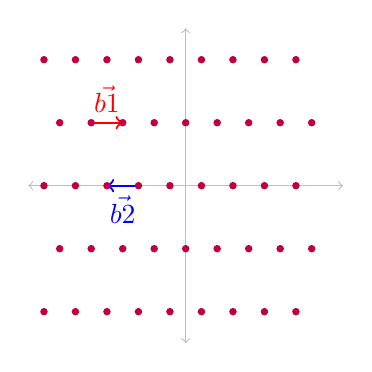
\begin{tikzpicture}[scale=.4]
\draw [lightgray] [<->] (0, 5) -- (10, 5);
\draw [lightgray] [<->] (5, 10) -- (5, 0);

% Vector
\draw[->, thick, red] (2, 7) -- (3, 7) node[midway, above, sloped] {$\vec{b1}$};
\draw[->, thick, blue] (3.5, 5) -- (2.5, 5) node[midway, below, sloped] {$\vec{b2}$};

% Các điểm không đều
\foreach \x/\y in {
0.5/1, 1/3, 1.5/1, 2/3, 2.5/1, 3/3, 3.5/1, 4/3, 4.5/1, 5/3, 5.5/1, 6/3, 6.5/1, 7/3, 7.5/1, 8/3, 8.5/1, 9/3,
0.5/5, 1/7, 1.5/5, 2/7, 2.5/5, 3/7, 3.5/5, 4/7, 4.5/5, 5/7, 5.5/5, 6/7, 6.5/5, 7/7, 7.5/5, 8/7, 8.5/5, 9/7,
0.5/9, 1.5/9, 2.5/9, 3.5/9, 4.5/9, 5.5/9, 6.5/9, 7.5/9, 8.5/9
}
{
\draw [fill, purple] (\x, \y) circle [radius=0.1];
}
\end{tikzpicture}
\end{figure}

\end{column}
\end{columns}

\end{frame}
%%%%%%%%%%%%%%%%%%%%%%%%%%%%%%%%%%%%%%%%%%%%%%%%%%%%%%%